\documentclass[../main]{subfiles}
\begin{document}

\section{Final product}
\label{s:app}
The final product is a mobile app for Android smartphone that allow the users to save their \textbf{Points of Interest}, have a \textbf{social interaction} 
 thanks to the friendship request, see and share \textbf{Live Events} with their friends and receive recommendation about a nice place to visit.
The main fragment of the application are the \textbf{map} and the \textbf{main menu} showed in the next picture.
\begin{figure}[H]
    \centering
    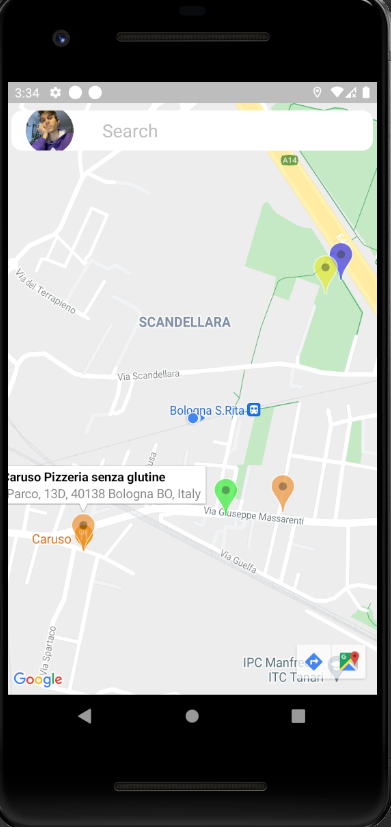
\includegraphics[width=70mm,height=150mm]{images/app/app_overview.png}
    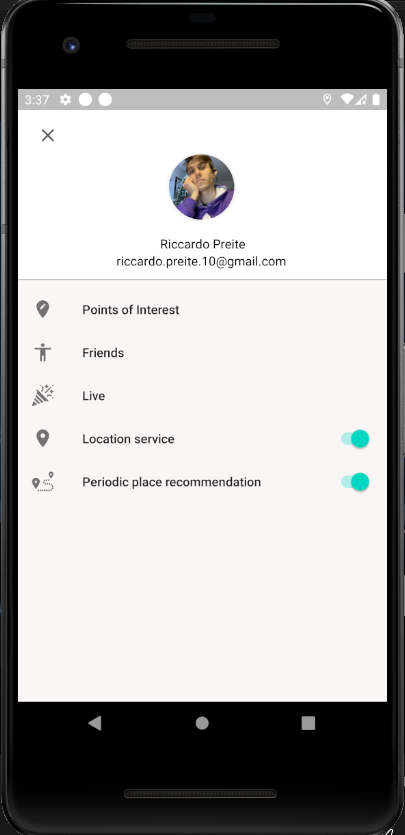
\includegraphics[width=70mm,height=150mm]{images/app/main_menu.png}
    \caption{On the left the map with some poi and on the right the main menu fragment.}
\end{figure}


\subfile{04_app/04_1_poi}
\subfile{04_app/04_2_friend}
\subfile{04_app/04_3_live}
\subfile{04_app/04_4_recommendation}

\end{document}